\chapter{Quantum Monte Carlo}
Many problems in nuclear physics involve a large number of particles in addition to a complicated interparticle interaction. The Schr\"odinger equation used to solve these problems involves a large dimensional integral with a complicated integrand. This is unfeasible to solve using standard numerical methods. Quantum Monte Carlo was designed to tackle these problems by sampling the large dimensional integrals in a way that reduces the necessary computation while still converging to an accurate answer. Without the fermion sign problem QMC calculations with an infinite number of samples are exact. Techniques are used to account for the sign and phase problems inherent in QMC calculations and with a sufficiently large number of samples the integrals can converge with controlled statistical errors. Two main ingredients to these QMC methods are Monte Carlo integration and the Metropolis algorithm. I will first describe these two techniques after which I will describe the QMC methods used in this work. I will then conclude by describing the Hamiltonians used with these methods. Useful references for all of the methods described herein include \cite{carlson2015, foulkes2001} and \cite{pederiva2017}.

\section{Monte Carlo Integration}
Calculating the properties of many-body quantum systems often involves solving a large dimensional integral such as
\begin{equation}
   I=\int g(\mathbf{R}) d\mathbf{R},
\end{equation}
where the $\mathbf{R}=\mathbf{r}_1,\mathbf{r}_2,\ldots,\mathbf{r}_A$ could be the positions of each nucleon in the system, and $A$ is the total number of nucleons. Monte Carlo integration involves writing this integral in terms of a probability distribution called the importance function $P(\mathbf{R})$,
\begin{equation}
   I=\int f(\mathbf{R}) P(\mathbf{R}) d\mathbf{R},
\end{equation}
where $f(\mathbf{R}) = g(\mathbf{R})/P(\mathbf{R})$. This integral is defined to be the expectation value of $f(\mathbf{R})$ with respect to the normalized importance function $P(\mathbf{R})$. The expectation value can also be determined by averaging an infinite number of $f(\mathbf{R}_n)$ where $\mathbf{R}_n$ are sampled directly from the importance function $P(\mathbf{R})$.
\begin{equation}
   I \equiv \left<f\right> = \lim\limits_{N\rightarrow\infty} \frac{1}{N} \sum\limits_{n=1}^N f(\mathbf{R}_n)
   \label{equ:mci}
\end{equation}
This expectation value can be approximated by averaging over a sufficiently large number of samples
\begin{equation}
   I \approx \frac{1}{N} \sum\limits_{n=1}^N f(\mathbf{R}_n),
\end{equation}
where the statistical uncertainties can be estimated in the usual way
\begin{equation}
   \sigma_{I} = \sqrt{\frac{\expect{f^2}-\expect{f}^2}{N}} \approx \sqrt{\frac{\left(\frac{1}{N}\sum\limits_{n=1}^Nf^2(\R_n)\right) - \left(\frac{1}{N}\sum\limits_{n=1}^Nf(\R_n)\right)^2}{N-1}}.
\end{equation}

The scaling is independent of the dimension, and thus this method is useful especially when the dimensions of the integration become large. In many-body quantum mechanics the dimension of the integrals can be quite large, including several dimensions for each particle in the calculation. Monte Carlo integration only needs to sample each of these dimensions, decreasing the work required by a substantial amount for large dimensional integrals.

\section{Metropolis Algorithm}
Monte Carlo integration requires the sampling of the importance function, $P(\R)$. This is straight forward only for functions that have a readily invertible cumulative distribution function, $F^{-1}(\R)$, which is not the case in our application. For the one dimensional case where $F^{-1}(x)$ is known, a random variables $x$ could be sampled by drawing a random variable $u$ from a uniform distribution from 0 to 1, which is then used as the argument of the inverse cumulative distribution function, $x=F^{-1}(u)$. The Metropolis algorithm provides a way to sample non-invertible probability distributions. The Metropolis algorithm is a Markov chain method that generates sequential samples of a probability distribution based on the previous sample alone, and not any other previous history. These are the steps to the algorithm.
\begin{enumerate}
   \item Start at a random position, $\R$.
   \item Propose a move to a new position $\R'$, sampled from a normalized distribution $T(\R'|\R)$. $T$ could be, for example, a Gaussian centered on the current position, but could be optimized for efficiency.
   \item The probability of accepting the move is given by enforcing a detailed balance condition. Alternative methods have been used for the acceptance condition including the heat bath method as described in \cite{sethna2006}.
   \begin{equation}
      A(\R'|\R) = \mathrm{min}\left(1, \frac{P(\R')T(\R|\R')}{P(\R)T(\R'|\R)}\right)
   \end{equation}
   \item A random number, $u$, is generated from a uniform distribution between 0 and 1, and the move is accepted if $A\ge u$, otherwise the original $\R$ is taken again as the sample.
\end{enumerate}

These steps are repeated until equilibrium is reached and all previous samples are discarded and only new samples are used. There are two conditions that need to be met to guarantee that this algorithm converges to the desired distribution. First, the transitions must be able to get from any allowed state to another in a finite number of steps. Second, the algorithm cannot include cycles between the same states. This second condition is guaranteed if there is a probability to reject transitions.

\section{Variational Monte Carlo}
Variational Monte Carlo starts with a trial wave function, $\psi_T$, that should have some non-zero overlap with the actual ground-state wave function, and a Hamiltonian, $H$. The trial wave function can be written as an expansion in the basis functions of the Hamiltonian, and will almost always include contributions from excited states of the system
\begin{equation}
   \Psi_T(\R) = c_0\Psi_0(\R) + \sum\limits_n c_n \Psi_n(\R).
\end{equation}
The expectation value of the Hamiltonian in the trial state gives what is called the variational energy. Due to the overlap with excited states the variational principle guarantees that the variational energy will be an upper bound to the true ground-state wave function as long as the trial wave function obeys the true symmetries of the system
\begin{equation}
   E_V = \frac{\int\psi_T^*(\R)H\psi_T(\R)d\R}{\int\psi_T^*(\R)\psi_T(\R)d\R} \ge E_0.
\end{equation}
For example a lower energy might be obtained by a wave function with a symmetric part, however the fermionic antisymmetry of the wave function is enforced. Other symmetries of the system are enforced including charge, particle number, and total angular momentum. This can be useful to calculate energies of different angular momentum states.


This integral is calculated using Monte Carlo integration and so it needs to be rewritten to match the form of Equation~\ref{equ:mci}. One way to get it into this form is to multiply and divide the numerator by $\psi_T^*(\R)\psi_T(\R)$ which gives
\begin{equation} 
  E_V = \int P(\R) E_L(\R) d\R,
\end{equation}
where
\begin{equation}
   P(\R) = \frac{|\Psi_T(\R)|^2}{\int|\Psi_T(\R)|^2d\R},
\end{equation}
\begin{equation}
   E_L(\R) = \frac{\Psi_T^*(\R)H\Psi_T(\R)}{\Psi_T^*(\R)\Psi_T(\R)},%E_L(\R) = \Psi_T^{-1}(\R) H \Psi_T(\R),
\end{equation}
are the importance function and local energy respectively.

Using the metropolis algorithm, a set of random configurations, $\{\R_n: n=1,A\}$, can be drawn from the probability distribution $P(\R)$ and used to sample the local energy. These sampled configurations are called walkers and contain the positions and often the spins and isospins of each particle. The variational energy and corresponding statistical error are then given by,
\begin{equation} 
  E_V \approx \frac{1}{N} \sum\limits_{n=1}^N E_L({\R_n}),
\end{equation}
\begin{equation} 
  \sigma_{E_V} = \sqrt{\frac{\left<E_L^2\right>-\left<E_L\right>^2}{N}} \approx \sqrt{\frac{\left(\frac{1}{N}\sum\limits_{n=1}^NE_L^2(\R_n)\right) - \left(\frac{1}{N}\sum\limits_{n=1}^NE_L(\R_n)\right)^2}{N-1}}
\end{equation}

The above description holds true for all spin-isospin dependent interactions. If the Hamiltonian depends on spin and isospin, which it does in nuclear physics, either the spin-isospin states can be explicitly summed over or the spin-isospin states can be sampled. For the case where the spin-isospin states are sampled the variational energy is evaluated as
\begin{equation} 
  E_V = \int d\R \sum\limits_S P(\R,S) E_L(\R,S),
\end{equation}
where
\begin{equation}
   P(\R,S) = \frac{|\Psi_T(\R,S)|^2}{\int|\Psi_T(\R,S)|^2d\R},
\end{equation}
and
\begin{equation}
   E_L(\R,S) = \frac{\sum_{S'}\Psi_T^*(\R,S')H_{S',S}\Psi_T(\R,S)}{\Psi_T^*(\R,S)\Psi_T(\R,S)},
\end{equation}
where the spin-isospin dependent Hamiltonian, $H_{S',S}$ can take a spin state from $S$ to $S'$. In the case where the spin-isospin states are explicitly summer over, the sums over states $S$ are done directly in the importance function and local energy, removing their explicit spin-isospin dependence.

Once evaluated the variational energy will be an upper bound to the ground state energy of the system. The $\Psi_T(\R)$ is written in terms of variational parameters which are varied to minimize the variational energy. A minimum in the energy will be produced when $\Psi_T \rightarrow \Psi_0$. It is important to note however that the trial wave functions that we often use are not exactly the ground-state wave functions and so the energies that we produce are only the minimum energy for that form of the trial wave function. As such, it is important to start with the best trial wave function form possible. Also, this algorithm can converge to a local minimum, and so it is again important to start with a good initial trial wave function.

\subsection{Variational Optimization}
The goal of an optimization method is to update the variational parameters in a way that lowers the energy. There are various methods for doing this including the Newton method (\cite{casalegno2003,umrigar2005}), the Linear method \cite{toulouse2007}, and the Stochastic Reconfiguration (SR) method (\cite{casula2004,sorella2001,sorella2005}), which we have used in this work. For systems with a small number of parameters the SR method is not the most efficient, however, for systems with a large number of parameters SR is very efficient.

\section{Diffusion Monte Carlo}
Diffusion Monte Carlo (DMC) solves for the ground-state by letting the walkers diffuse in imaginary time. The Schr\"odinger equation
\begin{equation}
   H\Psi = i\hbar\frac{\partial\Psi}{\partial t},
\end{equation}
can be written in imaginary time by substituting $\tau=it/\hbar$. The resulting equation is a diffusion equation,
\begin{equation}
   H\Psi = -\frac{\partial\Psi}{\partial\tau},
   \label{equ:diffusion}
\end{equation}
where the wave function $\Psi$ is diffused with respect to $\tau$. By separating variables we can write the solution as eigenfunctions in spatial coordinates times an exponential in imaginary time where the energies have been shifted by a parameter, $E_0$ in order to control the normalization, $V\rightarrow V - E_0$ and $E_n \rightarrow E_n-E_0$.
\begin{equation}
   \Psi(\R,\tau) = \sum\limits_{n=0}^\infty c_n\phi_n(\R)e^{-\tau(E_n-E_0)}
\end{equation}
As the imaginary time grows the states with higher energy than the ground-state are exponentially damped. The parameter $E_0$ is adjusted to be close to the ground state energy, and thus any states with higher energy have a non-zero difference $E_n-E_0$ in the negative exponential. Thus as $\tau\rightarrow\infty$ only the ground-state remains,
\begin{equation}
   \lim\limits_{\tau\rightarrow\infty}\Psi(\R,\tau) = c_0\phi_0(\R).
\end{equation}

The limit, $\lim\limits_{\tau\rightarrow\infty}\Psi(\R,\tau) = \lim\limits_{\tau\rightarrow\infty}e^{-(H-E_0)\tau}\Psi(\R)$, cannot be computed directly and so the propagator is split into small steps in imaginary time. A complete set of states are inserted between the propagator and the wave function.
\begin{equation}
   \braket{\R'}{\Psi_T(\tau)} = \int d\R \bra{\R'}e^{-(H-E_0)\tau}\ket{\R}\braket{\R}{\Psi_T(0)}
\end{equation}

The propagator is broken up into $N$ short time propagators, $\dt = \tau/N$, and a complete set of states is inserted between each finite time propagator,
\begin{equation}
\begin{split}
   \braket{\R_N}{\Psi_T(\tau)} = \int d\R_0 \ldots d\R_{N-1} \bra{\R_N}e^{-(H-E_0)\Delta\tau}\ket{\R_{N-1}} \times \ldots \\
      \times \bra{\R_1}e^{-(H-E_0)\Delta\tau}\ket{\R_{0}} \braket{\R_0}{\Psi_t(0)},
\end{split}
\end{equation}
where $\R_N=\R'$ and $\R_0=\R$. This can be written more conveniently in the form
\begin{align}
   \braket{\R_N}{\Psi_T(\tau)} &= \int d\R_0 \ldots d\R_{N-1} \left[\prod\limits_{i=1}^N \bra{\R_i}e^{-(H-E_0)\Delta\tau}\ket{\R_{i-1}}\right] \braket{\R_0}{\Psi_t(0)} \\
   &= \int d\R_0 \ldots d\R_{N-1} \left[\prod\limits_{i=1}^N G(\R_i,\R_{i-1},\Delta\tau)\right] \braket{\R_0}{\Psi_t(0)},
\end{align}
where $G(\R',\R,\tau)=\bra{\R'}e^{-(H-E_0)\tau}\ket{\R}$, is often called the Green's function or the propagator. We cannot calculate the Green's function directly and so the kinetic and potential terms need to be broken up and calculated separately.
\begin{equation}
   G(\R',\R,\dt) = \bra{\R'}e^{-T\dt}e^{-(V-E_0)\dt}\ket{\R}
\end{equation}
This breakup is only accurate to $\mathcal{O}(\dt^2)$. With the use of the Trotter-Suzuki formula,
\begin{equation}
   e^{-\tau\left(\hat{A}+\hat{B}\right)} = e^{-\tau\hat{B}/2)}e^{-\tau\hat{A})}e^{-\tau\hat{B}/2)} + \mathcal{O}(\tau^3)
\end{equation}
the finite-time propagator can be written as
\begin{align}
   G(\R',\R,\dt) &= \bra{\R'}e^{-(V-E_0)\dt/2}e^{-T\dt}e^{-(V-E_0)\dt/2}\ket{\R} \\
   &= e^{(V(\R')+V(\R)-2E_0)\dt/2}\bra{\R'}e^{-T\dt}\ket{\R}.
\end{align}
This break up is equal to the original Green's function up to $\mathcal{O}(\dt^3)$. To minimize time step errors the step in imaginary time needs to be kept small.

The kinetic term is used to move the walkers and the potential term is used to speed up convergence via a branching algorithm. The kinetic term is given by
\begin{equation}
   G_0(\R',\R,\Delta \tau) = \bra{\R'}e^{-T\Delta \tau}\ket{\R},
\end{equation}
which can be written as a diffusion term
\begin{equation}
   G_0(\R',\R,\Delta \tau) = \left(\frac{m}{2\pi\hbar^2\Delta\tau}\right)^{3A/2}e^{-m(\R'-\R)^2/2\hbar^2\Delta\tau},
\end{equation}
where $A$ is the total number of nucleons.
The piece that contains the potential is used to give a weight which is used with the branching algorithm,
\begin{equation}
   w(\R') = e^{(V(\R')+V(\R)-2E_0)\dt/2}.
   \label{equ:branchweight}
\end{equation}
There are various ways to do the branch algorithm, however the simplest way is to make copies of each walker, where the number of copies for each walker that continues in the calculation is given by $\mathrm{int}(w(\R')+\xi)$, where $\xi$ is a uniform random number from $[0,1]$. This way walkers with a small weight will more often be removed from the calculation and walkers with high weights will multiply.
\begin{figure}[h!]
   \centering
   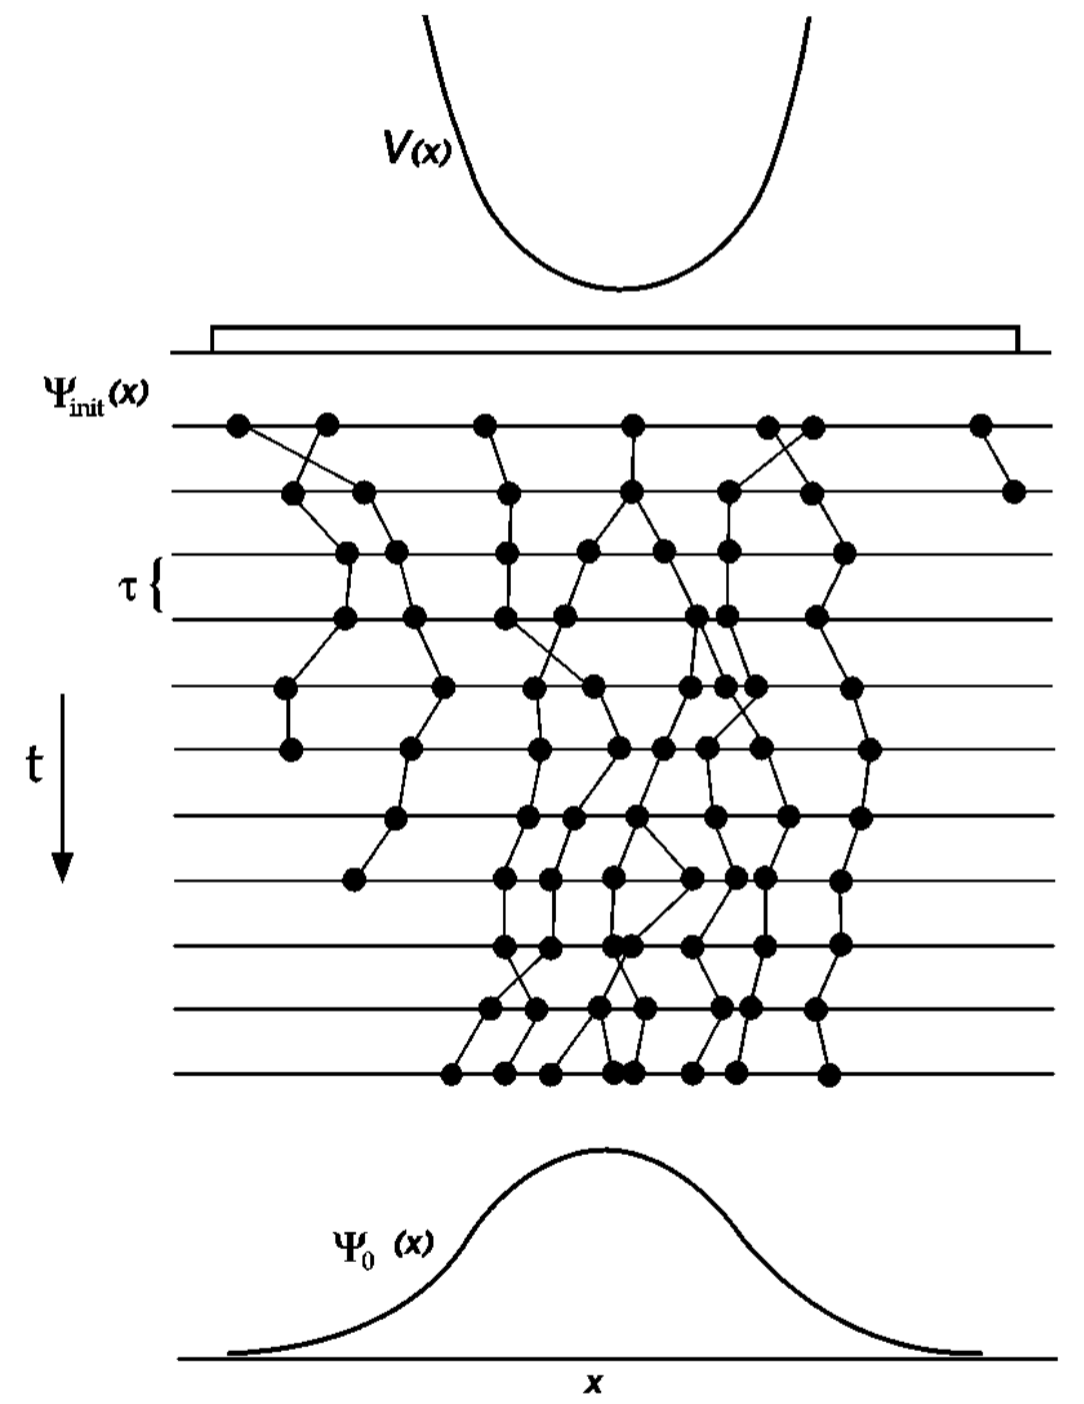
\includegraphics[width=0.4\textwidth]{figures/branching.png}
   \caption{Diagram describing the branching algorithm for Diffusion Monte Carlo (DMC). In this 1D example a particle is confined by the potential $V(x)$ and the trial wave function $\Psi_\text{init}(x)$ is propagated until it converges to the ground state wave function $\Psi_0(x)$. This diagram is from \cite{foulkes2001}.}
   \label{fig:branching}
\end{figure}

This sampling can have large uncertainties due to possible divergences in the branching weight in equation~\ref{equ:branchweight} as a result of particles getting too close or even coinciding. With the use of an importance function, $\Psi_I(\R)$ these fluctuations can be controlled without effecting the energy result. The importance function is used to bias the walker distributions toward $f(\R,t) = \Psi_T(\R,t)\Psi_I(\R)$ instead of $\Psi_T(\R,t)$ which effectively keeps the walkers away from locations where $\left|\Psi_T(\R,t)\right|^2$ is small.

This can be seen by multiplying Equation~\ref{equ:diffusion} by $\Psi_I(\R)$ and rewriting it in terms of $f(\R)$ as
\begin{equation}
   -\frac{1}{2}\nabla^2 f(\R,t) + \nabla\cdot\left[\mathbf{v}_D(\R) f(\R,t)\right] + \left[E_L(\R)-E_0\right]f(\R,t) = -\frac{\partial}{\partial t} f(\R,t),
\end{equation}
where $\mathbf{v}_D(R)$ is the drift velocity, defined as
\begin{equation}
   \mathbf{v}_D(\R) = \Psi_I(\R)^{-1}\nabla\Psi_I(\R) = \nabla \text{ln}\left|\Psi_I(\R)\right|.
\end{equation}
The drift velocity is responsible for pushing walkers away from areas of low $\left|\Psi_T(\R,t)\right|^2$. In practice the importance function is accounted for by directly sampling from
\begin{equation}
   G(\R',\R,\Delta\tau)\frac{\braket{\R}{\Psi_I}}{\braket{\R'}{\Psi_I}}
\end{equation}
instead of from the Green's function.

It is difficult to operate through the Green's function and so often observables are computed via mixed expectation values.
\begin{equation}
   \left<\mathcal{O(\tau)}\right>\text{mixed} = \frac{\bra{\Psi(\tau)}\mathcal{O}\ket{\Psi_T}}{\braket{\Psi(\tau)}{\Psi_T}}
\end{equation}
The true operator expectation value can approximately be written in terms of mixed expectation values \cite{pudliner1997} as
\begin{equation}
   \left<\mathcal{O(\tau)}\right> \approx 2\left<\mathcal{O(\tau)}\right>_\text{mixed} - \left<\mathcal{O}\right>_T,
   \label{equ:mixedexp}
\end{equation}
where
\begin{equation}
   \left<\mathcal{O}\right>_T = \frac{\bra{\Psi_T}\mathcal{O}\ket{\Psi_T}}{\braket{\Psi_T}{\Psi_T}}
\end{equation}
is the variational expectation value. Equation~\ref{equ:mixedexp} comes from a linear extrapolation of the mixed expectation value. For the Hamiltonian and operators that commute with the Hamiltonian the mixed expectation value is exactly the true expectation value for large time step. This can be seen directly with the Hamiltonian by splitting the Green's function up, to be used on either side of the Hamiltonian.
\begin{equation}
   \lim\limits_{\tau\rightarrow\infty}\left<H\right>_\text{mixed} = \frac{\bra{\Psi_T}e^{-H\tau/2}He^{-H\tau/2}\ket{\Psi_T}}{\bra{\Psi_T}e^{-H\tau/2}e^{-H\tau/2}\ket{\Psi_T}} = E_0
\end{equation}

The nuclear wave function is antisymmetric and will change sign as particle interact and exchange. As a result the oscillatory nature of the wave function requires positive and negative terms to cancel in the integral. Very accurate calculations must be done to accurately calculate these cancellations, and as a result very large uncertainties can be obtained. One approximate solution to this is the fixed-node approximation \cite{moskowitz1982}. The basic idea is that the trial wave function defines a nodal surface that is zero at the surface and changes sign across the surface. The wave functions are not allowed to cross the nodal surface. This maintains the upper bound principle of VMC, and is exact if the trial wave function, from which the nodal surface is defined, is exactly the ground state. This method assumes that the wave function is real, which is usually not the case with spin-isospin interactions. A generalization called the constrained path method works for real and complex wave functions alike \cite{wiringa2000}. The general idea is that walker configurations that have negative or zero overlap with the propagated wave function are discarded. This is only an approximate approach that depends on the choice of $\Psi_T(\R)$ and does not guarantee an upper bound on the energy. To this day there is active research looking for efficient ways to solve the Fermi-sign problem in many-body quantum systems. In practice we follow the method used in \cite{zhang2003} by using the real part of the trial wave function as the importance function and setting the weight to zero for any configuration whose overlap with the propagated wave function is zero or negative. This guarantees that the weights will be real and positive.

The constraint gives a non-exact result, however better convergence to the exact answer can be obtained by generating a set of good configurations with the constraint and then releasing the constraint for typically 20 to 40 steps to calculate the energy. Small systems, $A\le4$, will often converge before the statistical error overwhelms the signal. For larger systems an exponential extrapolation is typically used to determine the final energy as in \cite{pudliner1997}.

The DMC algorithm can generally be written as follows.
\begin{enumerate}
   \item Generate a set of random walkers. These are typically from the results of a VMC calculation, which has no constraint and provides an upper bound in the energy.
   \item For each walker propose a move, $\R' = \R + \mathbf{\chi}$, where $\mathbf{\chi}$ is a vector of random numbers from the shifted Gaussian $\exp\left(\frac{m}{2\hbar^2\Delta\tau}\left(\R'-\R+2\frac{\nabla\Psi_I(\R')}{\Psi_I(\R')}\right)^2\right)$.
   \item For each walker calculate the weight $w(\R')=\exp\left(-\left(\frac{E_L(\R')+E_L(\R)}{2}-E_0\right)\Delta\tau\right)$.
   \item Do branching.
   \item Calculate and collect the observables and uncertainties needed and increase the imaginary time by $\Delta\tau$.
   \item Repeat steps 2 through 5 until the uncertainties are small enough.
\end{enumerate}

The uncertainties are calculated by block averaging. The data we generate is inherently autocorrelated because each step in the Markov chain depends on the last. This will underestimate the statistical error in our calculation. The idea of block averaging is to form blocks in our data such that the average over each block is not correlated with the last block. This gives us a good estimate for the statistical uncertainty. In practice the block size is chosen so that the error estimate will not increase as the block size is increased. This is illustrated in the sample data shown in Figure~\ref{fig:blockaverage}.
\begin{figure}[h!]
   \centering
   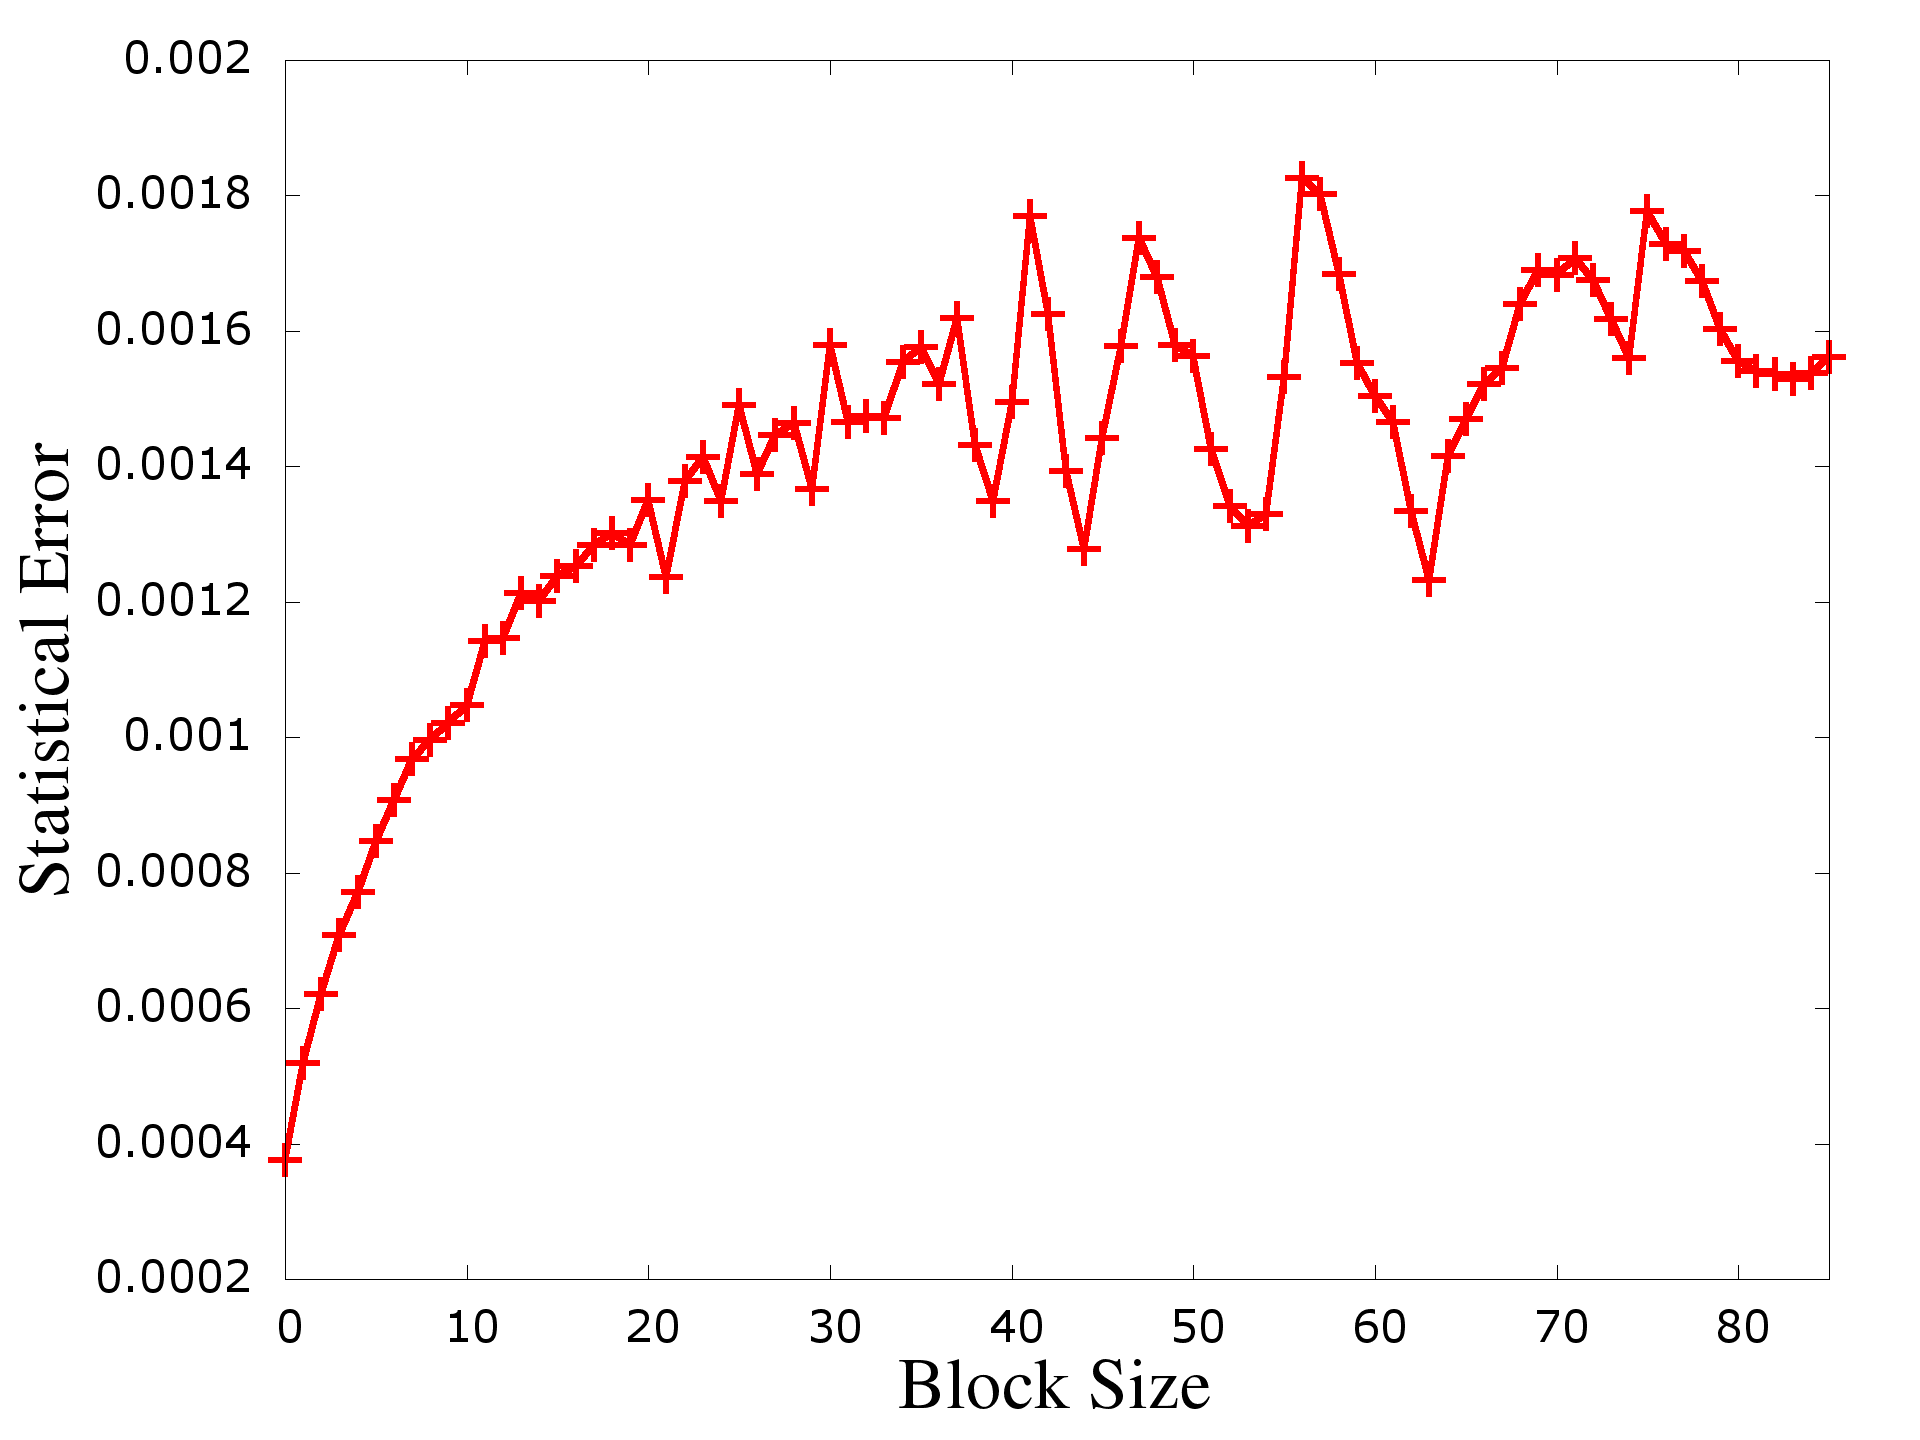
\includegraphics[width=0.7\textwidth]{figures/blockaverage.png}
   \caption{Sample data showing the convergence of the statistical uncertainty as the block size is increased. An appropriate block size for this data would be about 35, where the errors stop increasing with block size.}
   \label{fig:blockaverage}
\end{figure}

Good reviews of this method can be found in Refs. \cite{foulkes2001} and  \cite{carlson2015}. DMC only accounts for spin-isospin independent Hamiltonians, unlike Green's function Monte Carlo (GFMC) and auxiliary field diffusion Monte Carlo (AFDMC) which follow DMC for sampling spatial states but use two different methods to sample spin-isospin states. For each set of spatial integrals there is a sum over all of the spin and isospin states. GFMC evaluates this sum explicitly. This is inefficient as the number of spin states scales as
\begin{equation}
   \frac{A!}{Z!(A-Z)!}2^A
\end{equation}
where $A$ is the number of nucleons and $Z$ is the number of protons.
%The number of possible spin states given $A$ nucleons is $2^A$. The number of isospin states given $A$ nucleons and $Z$ protons can be reduced to ${A \choose Z}$ states leaving us with a total of $2^A {A \choose Z}$ spin-isospin states.
The number of states and the number of operators required for the trial wave function increase exponentially as the number of nucleons increases. To date, the largest nuclei that can be calculated with GFMC is ${}^{12}C$ \cite{lovato2013,lovato2014,lovato2015}. AFDMC was developed as an alternative to the explicit sum over spin-isospin states that GFMC performs.

\section{Auxiliary Field Diffusion Monte Carlo}
\label{sec:AFDMC}
To overcome the exponentially large number of spin-isospin states that have to be summed in GFMC, AFDMC was developed in 1999 \cite{schmidt1999} to sample spin and isospin states and, in analogy to moving the position of each walker, rotate the spin and isospin of each walker. The walkers are defined by the three spatial positions and amplitude for each particle to be in each of the four possible spin-isospin states $\ket{s} = \ket{p\uparrow,p\downarrow,n\uparrow,n\downarrow}$. The Hamiltonian can then be broken up into spin-isospin independent $H_{SI}$ and spin-isospin dependent $H_{SD}$ parts. The spin-isospin dependent part only comes from the potential and can be written as $V_{SD}$. The propagator can be broken up to have the old propagator used in DMC, which is independent of spin and isospin, and a spin-isospin dependent piece.
\begin{equation}
   G(\R'S',\R S,\tau)=\bra{\R'}e^{-(H-E_0)\tau}\ket{\R}G_{SD}(\R'S',\R S,\tau)
\end{equation}
where the spin-isospin dependent part of the propagator is
\begin{equation}
   G_{SD}(\R'S',\R S,\dt) = \bra {\R'S'}e^{-V_{SD}\dt} \ket{\R S}.
\end{equation}
The spin-isospin dependent part of the potential can be written as
\begin{equation}
   V_{SD} = \sum\limits_{p=2}^{M}\sum\limits_{i<j} \vpij\Opij,
\end{equation}
where M is the number of operators (e.g. $M=6$ for the AV6$'$ potential or $M=18$ for the Argonne AV18 two-body potential \cite{wiringa1984}). In this study I have used the standard AV6$'$ potential which includes the operators $\si\cdot\sj$, $\ti\cdot\tj$, $\si\cdot\sj \ti\cdot\tj$, $S_{ij}$ and $S_{ij} \ti\cdot\tj$, where $S_{ij} = 3\si\cdot\hat{r}_{ij}\sj\cdot\hat{r}_{ij}-\si\cdot\sj$. Here the $\mathbf{\si}$ and $\mathbf{\ti}$ operators are the Pauli matrices applied to spin and isospin of the $i$-th particle respectively.

AFDMC samples the spin and isospin states by expressing the operators in terms of squared single-particle particle operators which are transformed via the Hubbard-Stratanovich transformation. This can be done if the operators are expressed in the more convenient form
\begin{equation}
   V_{SD} = \frac{1}{2}\sum\limits_{i,\alpha,j,\beta} \sigma_{i,\alpha}A^{\sigma}_{i,\alpha,j,\beta}\sigma_{j,\beta}
      + \frac{1}{2}\sum\limits_{i,\alpha,j,\beta} \sigma_{i,\alpha}A^{\sigma\tau}_{i,\alpha,j,\beta}\sigma_{j,\beta}\ti\cdot\tj
      + \frac{1}{2}\sum\limits_{i,j} A^{\tau}_{i,j}\ti\cdot\tj,
   \label{equ:VwithA}
\end{equation}
where we have defined new $A$ matrices. The $A$ matrices are written in terms of the $\vpij$ functions above. For example the simplest matrix is the $A^{\tau}_{i,j}$ matrix which can be shown to be $A^{\tau}_{i,j} = v_{\tau}(r_{ij})$. There is a factor of one half in Eq.~\ref{equ:VwithA} because the sums go over all $i$ and $j$ particles instead of pairs for which $i<j$. These matrices are zero when $i=j$ and they are symmetric. We can also write these matrices in terms of their eigenvalues and eigenvectors.
\begin{align}
   &\sum\limits_{j,\beta} A^{\sigma}_{i,\alpha,j,\beta}\psi^{\sigma}_{n,j,\beta} = \lambda^{\sigma}_n\psi^{\sigma}_{n,i,\alpha} \\
   &\sum\limits_{j,\beta} A^{\sigma\tau}_{i,\alpha,j,\beta}\psi^{\sigma\tau}_{n,j,\beta} = \lambda^{\sigma\tau}_n\psi^{\sigma\tau}_{n,i,\alpha} \\
   &\sum\limits_{j} A^{\tau}_{i,j}\psi^{\tau}_{n,j} = \lambda^{\tau}_n\psi^{\tau}_{n,i}
\end{align}
Written in terms of these eigenvalues and eigenvectors the potential can be written as
\begin{equation}
   V_{SD} = \frac{1}{2}\sum\limits_{n=1}^{3A} \left(O_{n}^{\sigma}\right)^2 \lambda_n^{\sigma}
      + \frac{1}{2}\sum\limits_{\alpha=1}^{3}\sum\limits_{n=1}^{3A} \left(O_{n\alpha}^{\sigma\tau}\right)^2 \lambda_n^{\sigma\tau}
      + \frac{1}{2}\sum\limits_{\alpha=1}^{3}\sum\limits_{n=1}^{A} \left(O_{n\alpha}^{\tau}\right)^2 \lambda_n^{\tau},
\end{equation}
where the operators are given by
\begin{equation}
\begin{split}
   O_{n}^{\sigma} &= \sum\limits_{j,\beta} \sigma_{j,\beta}\psi_{n,j,\beta}^{\sigma} \\
   O_{n\alpha}^{\sigma\tau} &= \sum\limits_{j,\beta} \tau_{j,\alpha}\sigma_{j,\beta}\psi_{n,j,\beta}^{\sigma\tau} \\
   O_{n\alpha}^{\tau} &= \sum\limits_{j} \tau_{j,\alpha}\psi_{n,j}^{\tau}.
\end{split}
\end{equation}
These operators in the propagator now have the effect of rotating the spinors, analogous to diffusing the walkers in space. To reduce the order of the operators in the propagator from quadratic to linear we use the Hubbard-Stratanovich transformation.
\begin{equation}
   e^{-\frac{1}{2}\lambda O^2} = \frac{1}{\sqrt{2\pi}} \int dx e^{-\frac{x^2}{2} + \sqrt{-\lambda}x O}
\end{equation}
The variable $x$ is called an auxiliary field. Using the fact that there are $3A$ $O_{n}^{\sigma}$ operators, $9A$ $O_{n\alpha}^{\sigma\tau}$ operators and $3A$ $O_{n\alpha}^{\tau}$ operators, for a total of $15A$ operators, and by using the Hubbard-Stratanovich transformation we can write the spin-isospin dependent part of the propagator as
\begin{equation}
   G_{SD}(\R'S',\R S,\dt) = \bra{\R'S'}\prod\limits_{n=1}^{15A}\frac{1}{\sqrt{2\pi}}\int dx_n e^{-\frac{x_n^2}{2}}e^{\sqrt{-\lambda_n\dt} x_nO_n}\ket{\R S}.
   \label{equ:GSD}
\end{equation}
The spinors are rotated based on auxiliary fields sampled from the Gaussian with unit variance in Eq.~\ref{equ:GSD}. The sampling of the auxiliary fields is done in exactly the same way as the sampling of the spatial walkers in DMC, with the Markov chain Metropolis algorithm. Each sampled auxiliary field depends only on the previous sample and no more history than that.

Importance sampling can be included in the Auxiliary Field sampling in a similar way as described before with DMC. However, in practice it is done as follows. The $\Delta \R$ and $\Delta x_n$ are sampled by symmetric Gaussians and so the probability of $\Delta \R$ and $-\Delta \R$, and $\Delta x_n$ and $-\Delta x_n$ are the same. As a result the weight for the four possible combinations are sampled as
\begin{align}
   w_1 &= \frac{\braket{\Psi_I}{\R+\Delta \R, S'(x_n)}}{\braket{\Psi_I}{\R S}} e^{\left(-V_{SI}(\R+\Delta\R) - E_0\right)\dt} \\
   w_2 &= \frac{\braket{\Psi_I}{\R-\Delta \R, S'(x_n)}}{\braket{\Psi_I}{\R S}} e^{\left(-V_{SI}(\R-\Delta\R) - E_0\right)\dt} \\
   w_3 &= \frac{\braket{\Psi_I}{\R+\Delta \R, S'(-x_n)}}{\braket{\Psi_I}{\R S}} e^{\left(-V_{SI}(\R+\Delta\R) - E_0\right)\dt} \\
   w_4 &= \frac{\braket{\Psi_I}{\R-\Delta \R, S'(-x_n)}}{\braket{\Psi_I}{\R S}} e^{\left(-V_{SI}(\R-\Delta\R) - E_0\right)\dt},
\end{align}
and the sample with the largest weight is used. The weight for the chosen configuration, which is used for branching, is the average of the four weights
\begin{equation}
   W = \frac{1}{4}\sum\limits_{n=1}^4 w_n.
\end{equation}

\section{Hamiltonian}
One of the difficulties in many-body nuclear physics is finding an accurate Hamiltonian that is easy to calculate with the method you have selected. For QMC methods the Hamiltonian must be in configuration space and it must be local. Small degrees of non-locality can be addressed \cite{lynn2012,lynn2013}. Also, the nuclear physics Hamiltonian must be able to account for 2-body and 3-body interactions. The most generic form for the nuclear Hamiltonian then takes the form
\begin{equation}
   H = -\frac{\hbar^2}{2m}\sum\limits_i \nabla_i^2 + \sum\limits_{i<j} v_{ij} + \sum\limits_{i<j<k} V_{ijk} + \ldots.
\end{equation}
In principle there could be higher order terms included the in practice the two-nucleon NN interaction $v_{ij}$ and the three-nucleon interaction (TNI) $V_{ijk}$ are the only terms included as the importance of an $n$-nuclear potential decreases as $n$ increases. Calculations with only NN potentials will often underbind nuclei with $A>2$ and it has been shown that the inclusion of the TNI interaction improves this underbinding as well as level ordering in the excitation spectra of nuclei. This improvement has been shown in GFMC \cite{fantoni2008} as well as other methods such as the no-core shell model \cite{navratil2003}.

The NN potential takes the form
\begin{equation}
   v_{ij} = \sum\limits_{p=1}^M v_p(\r_{ij})\mathcal{O}^p_{ij},
\end{equation}
where $M$ is the number of operators begin used.
Two-nucleon potentials are often fit to NN scattering data and several very accurate models have been developed including the Nijmengen \cite{nagels1975,stoks1994}, CD-Bonn \cite{machleidt1996,machleidt2001}, and Argonne $v$18 (AV18) potentials \cite{wiringa1984,wiringa1995}. The Argonne potential is one of the most accurate and will be used in this work. The AV18 potential has 18 operators coming from one- and two-pion exchange as well as phenomenological sources. Often a subset of the AV18 potential is used, e.g. AV4$'$, AV6$'$, AV8$'$ or AV14$'$. These AV$n'$ potentials have kept only the top $n$ most important terms and are refit to scattering data at that level. A study of the successive importance of these terms up to $n=8$ compared with the full AV18 with and without three-nucleon potentials is given in \cite{wiringa2002}. The operators of the AV18 potential are
\begin{align}
   \mathcal{O}_{ij}^{p=1,8} &= \left[1,\si\cdot\sj,S_{ij},\mathbf{L}\cdot\mathbf{S}\right]\otimes\left[1,\ti\cdot\tj\right], \\
   \mathcal{O}_{ij}^{p=9,14} &= \left[\mathbf{L}^2,\mathbf{L}^2\si\cdot\sj,(\mathbf{L}\cdot\mathbf{S})^2\right]\otimes\left[1,\ti\cdot\tj\right], \\
   \mathcal{O}_{ij}^{p=15,18} &= \left[T_{ij},\si\cdot\sj T_{ij},S_{ij}T_{ij},\tau_i^2+\tau_j^2\right],
\end{align}
where the tensor term is $S_{ij} = 3\si\cdot\hat{r}_{ij}\sj\cdot\hat{r}_{ij}-\si\cdot\sj$, the $\mathbf{L}\cdot\mathbf{S}$ term is the spin-orbit term, and the $T_{ij} = 3\tau_i^2\tau_j^2-\ti\cdot\tj$ is the isotensor term.

In this work the AV6$'$ potential is used, which includes all of the same operators as AV8$'$ except for those including the spin-orbit terms, $\left[1,\si\cdot\sj,S_{ij}\right]\otimes\left[1,\ti\cdot\tj\right]$. The functions multiplying the AV6$'$ operators are shown in figure \ref{fig:vij}.
\begin{figure}[h!]
   \centering
   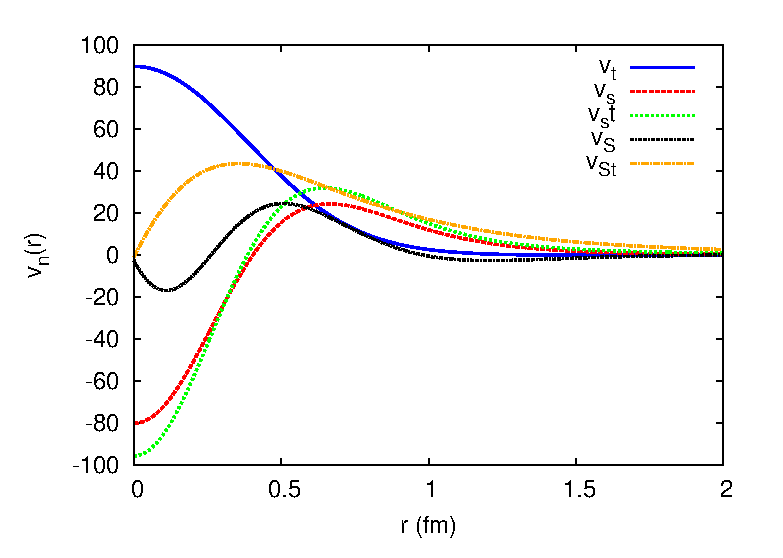
\includegraphics[width=0.7\textwidth]{figures/vij.eps}
   \caption{The functions multiplying the AV6$'$ operators as a function of nucleon separation. The central operator is excluded to show the spin-isospin terms with better detail. The $v_s$ represents the spin operators, $v_t$ the isospin operators, $v_{st}$ the spin-isospin operators, $v_S$ the tensor, and $v_{St}$ the tensor-isospin operators.}
   \label{fig:vij}
\end{figure}

The AV6$'$ can be broken up in Cartesian coordinates including 39 operators, 3 from $\tau$, 9 from $\sigma$, and 27 from $\sigma\tau$ terms. This can be done by writing the potential in the form
\begin{equation}
   \sum\limits_p v_p(\r_{ij})\mathcal{O}^p_{ij} = v_1(\r_{ij}) + \sum\limits_\alpha \t_{i\alpha}A^\tau_{ij}\t_{j\alpha} + \sum\limits_{\alpha,\beta} \s_{i\alpha}A^\sigma_{ij}\s_{j\beta} + \sum\limits_{\alpha,\beta,\gamma} \s_{i\alpha}\t_{i\gamma}A^{\sigma\tau}_{ij}\s_{j\beta}\t_{j\gamma},
\end{equation}
where the matrices are given by
\begin{align}
   A^\tau_{ij} &= v_2(\r_{ij}), \\
   A^\sigma_{ij} &= v_3(\r_{ij})\delta_{\alpha\beta} + v_5(\r_{ij})(3\rij^\alpha\rij^\beta-\delta_{\alpha\beta}), \\
   A^{\sigma\tau}_{ij} &= v_5(\r_{ij})\delta_{\alpha\beta} + v_6(\r_{ij})(3\rij^\alpha\rij^\beta-\delta_{\alpha\beta}).
\end{align}
This is a simple way to break up the AV6$'$ potential but a more efficient breakup can be used in which only 15 operators are needed. This is achieved by using $\rij$ as the first basis function and then using two additional orthogonal basis functions. This reduces the $\rij^\alpha\rij^\beta$ term in the matrices to $\delta_{\alpha\beta}$. This potential can then be written as
\begin{equation}
   \sum\limits_p v_p(\r_{ij})\mathcal{O}^p_{ij} = v_1(\r_{ij}) + \sum\limits_\alpha \t_{i\alpha}A^\tau_{ij}\t_{j\alpha} + \sum\limits_{\alpha} \s_{i\alpha}A^\sigma_{ij}\s_{j\alpha} + \sum\limits_{\alpha,\gamma} \s_{i\alpha}\t_{i\gamma}A^{\sigma\tau}_{ij}\s_{j\alpha}\t_{j\gamma},
\end{equation}
where the matrices are given by
\begin{align}
   A^\tau_{ij} &= v_2(\r_{ij}), \\
   A^\sigma_{ij} &= v_3(\r_{ij}) + 2v_5(\r_{ij}), \\
   A^{\sigma\tau}_{ij} &= v_5(\r_{ij}) + 2v_6(\r_{ij}),
\end{align}
where it is easy to see that there are 3 $\tau$, 3 $\sigma$, and 9 $\sigma\tau$ terms for a total of 15 operators in this basis.

Calculations with $A\le2$ are well described by the NN potentials, however for any system with $A\ge3$ the 3-nucleon force is needed to accurately describe the system. The phenomenological 3-nucleon forces that are typically employed in AFDMC calculations are the older Urbana and newer Illinois potentials. The Urbana IX (UIX) potential is built using the two-pion three-nucleon interaction, which can be written as
\begin{equation}
\begin{split}
   V_{2\pi3N} = \sum\limits_\text{cycl.} &A_{2\pi}\{\t_1\cdot\t_2,\t_1\cdot\t_3\} \{(S_{12}T(\r_{12})+\s_1\cdot\s_2 Y(\r_{12})),(S_{13}T(\r_{13})+\s_1\cdot\s_3 Y(\r_{13}))\} \\
      + &C_{2\pi}\left[\t_1\cdot\t_2,\t_1\cdot\t_3\right] \left[(S_{12}T(\r_{12})+\s_1\cdot\s_2 Y(\r_{12})),(S_{13}T(\r_{13})+\s_1\cdot\s_3 Y(\r_{13}))\right] \\
      + &B(\r_{12},\r_{13})\{\t_1\cdot\r_2,\t_1\cdot\t_3\}\{(S_{12}+\s_1\cdot\s_2),(S_{13}+\s_1\cdot\s_3)\},
\end{split}
\end{equation}
where the sum is a cyclic sum over 1, 2, and 3. The $\{~,~\}$ and $[~,~]$ are anticommutators and commutators and the $Y(r)$ and $Y(r)$ are the radial Yukawa and one-pion exchange interactions as described in \cite{carlson1983},
\begin{align}
   Y(r) &= \frac{e^{-\mu r}}{\mu r} Y_\text{cut}(r) \\
   T(r) &= \left(1+\frac{3}{\mu r} + \frac{3}{\mu^2 r^2}\right)\frac{e^{-\mu r}}{\mu r} T_\text{cut}(r),
\end{align}
where $Y_\text{cut}(r)$ and $T_\text{cut}(r)$ are the cutoff functions for the Yukawa and one-pion exchange terms respectively. The $B(\r_{12},\r_{13})$ term comes from $\pi$N s-wave scattering. The UIX potential is fit to the ground states of $^3$H and $^4$He. For details about the construction and results obtained with this potential I refer the reader to \cite{carlson1983, pudliner1996, pudliner1997}.

The Illinois-7 (IL7) potential \cite{pieper2001} contains two-pion three-nucleon interactions in both the s-wave and p-wave, as well as a three-pion exchange and three-nucleon contact interactions. The IL7 potential has been fit to the low-lying spectra of nuclei with $A=3$ to nuclei with $A=10$. These phenomenological potentials have been used to calculate many properties of light nuclei with high accuracy using both the GFMC and AFDMC methods.

Despite the accuracy of these potentials they have little direct connection to the underlying theory of QCD. In recent years a set of nuclear potentials has been developed from a chiral effective field theory ($\chi$EFT) framework that can be used with nuclear QMC methods such as GFMC and AFDMC \cite{epelbaum2009,machleidt2011}. These potentials are local up the next-to-next-to leading order (N$^2$LO) and so QMC calculations can use potentials up to this order. Good results using these potentials have been obtained with both GFMC \cite{lynn2014} and AFDMC \cite{lonardoni2018}.

All calculations here have been done with the AV6$'$ potential to reduce computation requirements as well as to better focus on the improvements made by improved wave functions. It would be straightforward to do any of these calculations with the three-nucleon and the $\chi$EFT potentials.
